\documentclass[a4paper,american]{paper}
\usepackage[T1]{fontenc}
\usepackage[utf8]{inputenc}
\pagestyle{plain}
\usepackage{babel}
\usepackage{textcomp}
\usepackage{amsmath}
\usepackage{amsthm}
\usepackage{setspace}
\usepackage[unicode=true]{hyperref}
\usepackage{breakurl}
\usepackage{txfonts}
\usepackage{pxfonts}
\usepackage{tikz}
\usetikzlibrary{arrows.meta,positioning,calc}
\usepackage{tkz-graph}
\usepackage{graphicx}
\usepackage{float}
\usepackage{needspace}

\graphicspath{ {./images/} }

\makeatletter
\providecommand*{\code}[1]{\texttt{#1}}
\makeatother

\begin{document}

\title{An interactive demonstration of counterfactual truth conditions%
	\footnote{Further title proposals:
		(B) Creating an educational computer game about counterfactuals in terms of a centered system of spheres
		(C) Implementing a computer game illustrating the truth conditions of counterfactuals as variably strict conditionals
	}
}

\subtitle{Proposal for a Bachelor Thesis (v0.4, 8 Juli 2022)}

\author{%
	Andreas Paul Bruno Lönne\\
	\code{\href{mailto:loenne@campus.tu-berlin.de}{loenne@campus.tu-berlin.de}}
}

\institution{
	Technische Universität Berlin\\discourse
	Degree program: Bachelor Informatik / Computer Science
}

\maketitle

\section*{Problem: An approachable showcase of counterfactuals}
{\it Counterfactuals} are in essence conditional statements carrying information about the relationship of a false {\it antedecent} and a {\it consequent}. Their truth value answers the question: ``If it were the case that A, would it then be the case that B?''. {\it Counterfactual~thought}---that is the thought of alternate outcomes---\cite{byrne_counterfactual_thought_2016} is common for humans to engage in and is consequently subject to a great volume of philosophical and mathematical discourse. 

Considering the amount of information available and the various propositions on how to mathematically model counterfactuals \cite{stalnaker_theory_1968, stalnaker_semantic_1970,  lewis_counterfactuals_1973}, gaining an understanding of the nuances of counterfactual truth conditions tends to be a difficult endeavour for any layman. I propose to remedy this issue by implementing a computer game based on a semantic game of counterfactuals.

\section*{Approach: A computer game on counterfactuals}
The aforementioned semantic game of counterfactuals expresses the evaluation of {\it Lewis's~counterfactual~truth~conditions} \cite{lewis_counterfactuals_1973} in terms of a two-player game wherein a defender tries to prove a counterfactual sentence and an attacker attempts to disprove it.

The game state is described by a tuple holding a counterfactual sentence $\varphi$ and a world $w$ at which $\varphi$ ought to be shown. Additionally the subscript of a tuple denotes whose players turn it is. Tuples with designators "vac" and "cf" are exceptions to that syntax, indicating supposed vacuous truth or truth at all worlds at least as similar to $w$ as $w'$. Here are some examples:

\begin{center}
$(\varphi ,w)_{d/a},\hspace{5px}(vac,\varphi ,w)_a,\hspace{5px}(cf,\varphi ,\psi ,w,w',r)_a$
\end{center}

The constituents of a counterfactual sentence~$\varphi$ are negations~$\neg$, disjunctions~$\vee$, the counterfactual~would~operator~$\boxright$, the bottom symbol~$\bot$ and atomic statements. To be able to resolve atomic statements each world $w$  has a set of true atomic statements $F(w)$ associated with it. Moreover a {ternary~relation~$\leadsto$} expresses similarity between worlds from the standpoint of one world.

Given those remarks, the concrete rules of the game are as stated in figure~\ref{fig:rules}.

\section*{Approach: Visual representation}

I intend to create a software solution that is intuitive and easy to use. The user is meant to be able to learn about counterfactuals, with little prior knowledge or time investment. Hence a minimalistic and functional user interface has to be developed.

For the purposes of visual clarity, usability and simplicity the application will provide finite selections of exemplar worlds as stand-ins for potentially infinite sets of accessible worlds and visualize them as nodes of a graph as shown in figure \ref{fig:closest_worlds}.

\begin{figure}[H]
	\centering
	\begin{tikzpicture}[main/.style = {draw, circle}]	
	\node[inner sep=0pt] (1)  at (0,0) {
\includegraphics[width=.0725\textwidth]{5FactsEath.png}};
	\node[inner sep=0pt] (2)  at (2,1) {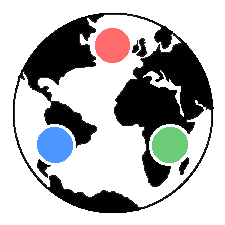
\includegraphics[width=.0725\textwidth]{3FactsEath.png}};
	\node[inner sep=0pt] (3)  at (-2,1) {
\includegraphics[width=.0725\textwidth]{1FactEath.png}};
	\node[inner sep=0pt] (4)  at (-1,-2) {
\includegraphics[width=.0725\textwidth]{4FactsEath.png}};
	\node[inner sep=0pt] (5)  at (2,-2) {
\includegraphics[width=.0725\textwidth]{3Facts2Eath.png}};
	
	\path [->] let \p1=($(2)-(1)$),\n1={atan2(\y1,\x1)},\n2={180+\n1} in
     ($ (1.\n1)!6pt!90:(2.\n2) $) edge node[midway,fill=white] {$1$} ($ (2.\n2)!6pt!-90:(1.\n1) $);
    \path [->] let \p1=($(1)-(2)$),\n1={atan2(\y1,\x1)},\n2={180+\n1} in
     ($ (2.\n1)!6pt!90:(1.\n2) $) edge node[midway,fill=white] {$2$} ($ (1.\n2)!6pt!-90:(2.\n1) $);
	
	\path [->] let \p1=($(3)-(1)$),\n1={atan2(\y1,\x1)},\n2={180+\n1} in
     ($ (1.\n1)!6pt!90:(3.\n2) $) edge node[midway,fill=white] {$3$} ($ (3.\n2)!6pt!-90:(1.\n1) $);
    \path [->] let \p1=($(1)-(3)$),\n1={atan2(\y1,\x1)},\n2={180+\n1} in
     ($ (3.\n1)!6pt!90:(1.\n2) $) edge node[midway,fill=white] {$2$} ($ (1.\n2)!6pt!-90:(3.\n1) $);
     
     \path [->] let \p1=($(4)-(1)$),\n1={atan2(\y1,\x1)},\n2={180+\n1} in
     ($ (1.\n1)!6pt!90:(4.\n2) $) edge node[midway,fill=white] {$2$} ($ (4.\n2)!6pt!-90:(1.\n1) $);
    \path [->] let \p1=($(1)-(4)$),\n1={atan2(\y1,\x1)},\n2={180+\n1} in
     ($ (4.\n1)!6pt!90:(1.\n2) $) edge node[midway,fill=white] {$2$} ($ (1.\n2)!6pt!-90:(4.\n1) $);	
     
     \path [->] let \p1=($(5)-(1)$),\n1={atan2(\y1,\x1)},\n2={180+\n1} in
     ($ (1.\n1)!6pt!90:(5.\n2) $) edge node[midway,fill=white] {$1$} ($ (5.\n2)!6pt!-90:(1.\n1) $);
    \path [->] let \p1=($(1)-(5)$),\n1={atan2(\y1,\x1)},\n2={180+\n1} in
     ($ (5.\n1)!6pt!90:(1.\n2) $) edge node[midway,fill=white] {$4$} ($ (1.\n2)!6pt!-90:(5.\n1) $);	
     
     \path [->] let \p1=($(5)-(2)$),\n1={atan2(\y1,\x1)},\n2={180+\n1} in
     ($ (2.\n1)!6pt!90:(5.\n2) $) edge node[midway,fill=white] {$5$} ($ (5.\n2)!6pt!-90:(2.\n1) $);
    \path [->] let \p1=($(2)-(5)$),\n1={atan2(\y1,\x1)},\n2={180+\n1} in
     ($ (5.\n1)!6pt!90:(2.\n2) $) edge node[midway,fill=white] {$5$} ($ (2.\n2)!6pt!-90:(5.\n1) $);
     
     \path [->] let \p1=($(4)-(5)$),\n1={atan2(\y1,\x1)},\n2={180+\n1} in
     ($ (5.\n1)!6pt!90:(4.\n2) $) edge node[midway,fill=white] {$4$} ($ (4.\n2)!6pt!-90:(5.\n1) $);
    \path [->] let \p1=($(5)-(4)$),\n1={atan2(\y1,\x1)},\n2={180+\n1} in
     ($ (4.\n1)!6pt!90:(5.\n2) $) edge node[midway,fill=white] {$2$} ($ (5.\n2)!6pt!-90:(4.\n1) $);
     
    \draw[->] (1) to [out=110,in=70,looseness=4] node[above] {$0$} (1);
    \draw[->] (2) to [out=20,in=-20,looseness=4] node[right] {$0$} (2);
	\draw[->] (3) to [out=200,in=160,looseness=4] node[left] {$0$} (3);
	\draw[->] (4) to [out=200,in=160,looseness=4] node[left] {$0$} (4);
	
	\end{tikzpicture}
	\caption{similarity graph of exemplar worlds}
	\label{fig:closest_worlds}
\end{figure}

The directed edges of the graph express dissimilarity from the standpoint of one world to another. And the colored dots represent atomic statements from the set $F(w)$, that each world has associated with it.

Additionally I will determine a visual representation of counterfactual sentences from amongst various possibilities such as natural language, logical expressions and logical expression trees. While natural language is the most intuitive representation, it lacks the unambiguity of logical constructs and may create long unreadable sentences. Logical expressions, however, tend to be difficult to read and comprehend for laymen. Here are some examples of the same counterfactual statement expressed in different ways in (\ref{language}), (\ref{formula}) and figure~\ref{fig:exptree}.

\begin{align}
    \text{\parbox{11cm}{``If Alexander~the~Great had not died at the age of 32 and attacked europe, the Romans would have defeated him''}}
     \label{language}
\end{align}
\begin{equation}
	\neg(\varphi_1\vee\neg\varphi_2)\boxright\psi
	\label{formula}
\end{equation}

\begin{figure}[h]
	\centering
	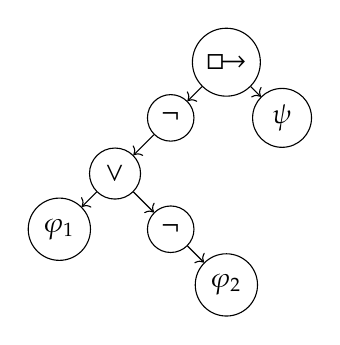
\begin{tikzpicture}[main/.style = {draw, circle}]
	\node[main] (1) {$\boxright$};
	\node[main] (2) [below left of=1] {$\neg$};
	\node[main] (3) [below right of=1] {$\psi$};
	\node[main] (4) [below left of=2] {$\vee$};
	\node[main] (5) [below left of=4] {$\varphi_1$};
	\node[main] (6) [below right of=4] {$\neg$};
	\node[main] (7) [below right of=6] {$\varphi_2$};
	
	\draw[->] (1) -- (2);
	\draw[->] (1) -- (3);
	\draw[->] (2) -- (4);
	\draw[->] (4) -- (5);
	\draw[->] (4) -- (6);
	\draw[->] (6) -- (7);

	
	\end{tikzpicture}
	\caption{counterfactual sentence as a logical expression tree}
	\label{fig:exptree}
\end{figure}

\section*{Method: Deployment as a lightweight web application}

In order to deliver an easily accessible software solution I intend to make use of the Phaser~3 Framework for Typescript to develop a web-application. Phaser~3 is well suited for this task because it is a lightweight framework, that fits the scope of the project and allows for distribution of the software with a small barrier to entry.

\section*{Rules of the semantic game}

\begin{figure}[H]
	\centering
	\begin{equation}
		(\bot ,w)_{d/a}\hspace{10pt}\text{Attacker wins}
	\end{equation}
	\begin{equation}
		(\neg\bot ,w)_{d/a}\hspace{10pt}\text{Defender wins}
	\end{equation}
	\begin{equation}
		(\varphi ,w)_{d/a}\xrightarrow{\varphi\in F(w)}(\neg\bot ,w)_{d/a}
	\end{equation}
	\begin{equation}
		(\varphi ,w)_{d/a}\xrightarrow{\varphi\not\in F(w)}(\bot ,w)_{d/a}
	\end{equation}
	\begin{equation}
		(\neg\varphi ,w)_{d/a}\xrightarrow{\varphi\in F(w)}(\bot ,w)_{d/a}
	\end{equation}
	\begin{equation}
		(\neg\varphi ,w)_{d/a}\xrightarrow{\varphi\not\in F(w)}(\neg\bot ,w)_{d/a}
	\end{equation}
	\begin{equation}
		(\neg\neg\varphi ,w)_{d/a}\rightarrow (\varphi ,w)_{d/a}
	\end{equation}
	\begin{equation}
		(\varphi\vee\psi ,w)_d\rightarrow (\varphi ,w)_{d/a}
	\end{equation}
	\begin{equation}
		(\varphi\vee\psi ,w)_d\rightarrow (\psi ,w)_{d/a}
	\end{equation}
	\begin{equation}
		(\neg (\varphi\vee\psi ),w)_a\rightarrow (\neg\varphi ,w)_{d/a}
	\end{equation}
	\begin{equation}
		(\neg (\varphi\vee\psi ),w)_a\rightarrow (\neg\psi ,w)_{d/a}
	\end{equation}
	\begin{equation}
		(\varphi\boxright\psi ,w)_d\rightarrow (vac,\varphi ,w)_a
	\end{equation}
	\begin{equation}
		(vac,\varphi ,w)_a\xrightarrow{[w\overset{r}{\leadsto}w']}(\neg\varphi ,w')_{d/a}
	\end{equation}
	\begin{equation}
		(\varphi\boxright\psi ,w)_d\xrightarrow{[w\overset{r}{\leadsto}w']}(cf,\varphi ,\psi ,w,w',r)_a
	\end{equation}
	\begin{equation}
		(cf,\varphi ,\psi ,w,w',r)_a\rightarrow (\varphi ,w')_{d/a}
	\end{equation}
	\begin{equation}
		(cf,\varphi ,\psi ,w,w',r)_a\xrightarrow{[w\overset{r^*}{\leadsto}w^*,r^*\leq r]}(\neg\varphi\vee\psi ,w^*)_d
	\end{equation}
	\begin{equation}
		(\neg (\varphi\boxright\psi ),w)_a\rightarrow (vac,\varphi ,w)_d
	\end{equation}
	\begin{equation}
		(vac,\varphi ,w)_d\xrightarrow{[w\overset{r}{\leadsto}w']} (\varphi ,w')_{d/a}
	\end{equation}
	\begin{equation}
		(\neg (\varphi\boxright\psi ),w)_a\xrightarrow{[w\overset{r}{\leadsto}w']}(cf,\varphi ,\psi ,w,w',r)_d
	\end{equation}
	\begin{equation}
		(cf,\varphi ,\psi ,w,w',r)_d\rightarrow(\neg\varphi ,w')_{d/a}
	\end{equation}
	\begin{equation}
		(cf,\varphi ,\psi ,w,w',r)_d\xrightarrow{[w\overset{r^*}{\leadsto}w^*, r^*\leq r]}(\neg(\neg\varphi\vee\psi ),w^*)_a
	\end{equation}
	\caption{rules of the semantic game of counterfactuals}
	\label{fig:rules}
\end{figure}

\Needspace{5\baselineskip}
\section*{Schedule}

In accordance with \href{https://www.eecs.tu-berlin.de/fileadmin/f4/fkIVdokumente/StuPOs/Informatik/Lesefassung_BSc_Informatik.pdf}{StuPO~Bachelor~Informatik 2015}, the elaboration of the thesis is scheduled over a period of 20 weeks:
\begin{description}
\item [3 weeks] Familiarization with theory \& Game design.
\item [1 week] Implementation of a semantic game engine. (Output: Software)
\item [3 weeks] Implementation of the user interface. (Output: Counterfactual representation, Graph representation, Menu)
\item [2 weeks] Creation of levels or levelgenerator. (Output: Software)
\item [2 weeks] Testing \& QA.
\item [6 weeks] Write thesis. (Output: Thesis)
\item [3 weeks] Puffer
\end{description}

\section*{Thesis Outline (Sketch)}

\begin{enumerate}
	\item Introduction
	\begin{enumerate}
		\item Problem description
		\item Context / related work
		\item Overview
	\end{enumerate}
	\item Formulation of the semantic game of counterfactuals
	\begin{enumerate}
		\item Definitions (worlds, facts at worlds, graph of worlds)
		\item Game rules
	\end{enumerate}
	\item Implementation
	\begin{enumerate}
		\item Design decisions (visual representation of cfs, finite graph / exemplar worlds)
		\item Discussion of the framework
		\item Implementation of the semantic game engine
		\item Evaluation of the implementation
	\end{enumerate}
	\item Conclusion
	\begin{enumerate}
		\item Summary
		\item Outlook
	\end{enumerate}
\end{enumerate}

\bibliographystyle{alphaurl}
\nocite{*}
\bibliography{expose}

\end{document}
